\documentclass{wileySix}
\usepackage{w-bookps}

% \usepackage{mathptmx}

\usepackage{graphicx}
\usepackage{enumitem}

\setcounter{secnumdepth}{3}

\setcounter{tocdepth}{2}

\begin{document}

\booktitle{Sistem Operasi}
\subtitle{Semua Tentang Sistem Operasi}

\author{Rolly Maulana Awangga}

\halftitlepage
\titlepage



\offprintinfo{Sistem Operasi, pre-release}{Rolly Maulana Awangga}


\begin{copyrightpage}{2018}
Web Service / Rolly Maulana Awangga
\end{copyrightpage}


\dedication{For my family}

\contentsinbrief %optional
\tableofcontents
\listoffigures %optional
\listoftables  %optional

%%%%%%%%%
%%Content 
%%%%%%%%%

\part[Pengenalan Sistem Operasi]
{Pengenalan\\ Sistem Operasi}

\chapter[Contoh]
{Contoh\\ Latex}
\prologue{The sheer volumne of answers can often stifle insight...The purpose
of computing\index{computing!the purpose} is insight, not numbers.}
{Hamming}

\section{Definisi}
Sistem Informasi Geografis merupakan penggalan kata dan Sistem Informasi dan Geografis. Geografis dipandang sebagai bentukan dari geospasial.
Geospasial memiliki arti geo yang berarti bumi dan spasial yang berarti ruang atau keruangan. Jadi geospasial merupakan ilmu yang mempelajari 
tata ruang dari bumi. Tata ruang melingkupi letak suatu titik di bumi baik itu letak kota, provinsi atau negara. Tata ruang juga menyajikan gambaran dari ruang tersebut yang disebut dengan ilmu kartografi atau sering disebut sebagai ilmu pembuatan peta\cite{awangga2017colenak}.

\section{Sejarah Peta}
Perkembangan peta dunia tidak luput dari para ahli geografi dan kartografi. Peta dunia yang populer pada saat ini merupkan kontribusi dari para 
pembuat peta sebelumnya

\subsection{Ptolemy's}
Ptolemy's diduga membuat peta pada abad ke 2


\subsection{Muhammad al-Idrisi}
Seorang ahli geografi dan kartografi Muhammad al-Idrisi membuat peta dunia pada abad ke 11

\begin{figure}[ht]

\centerline{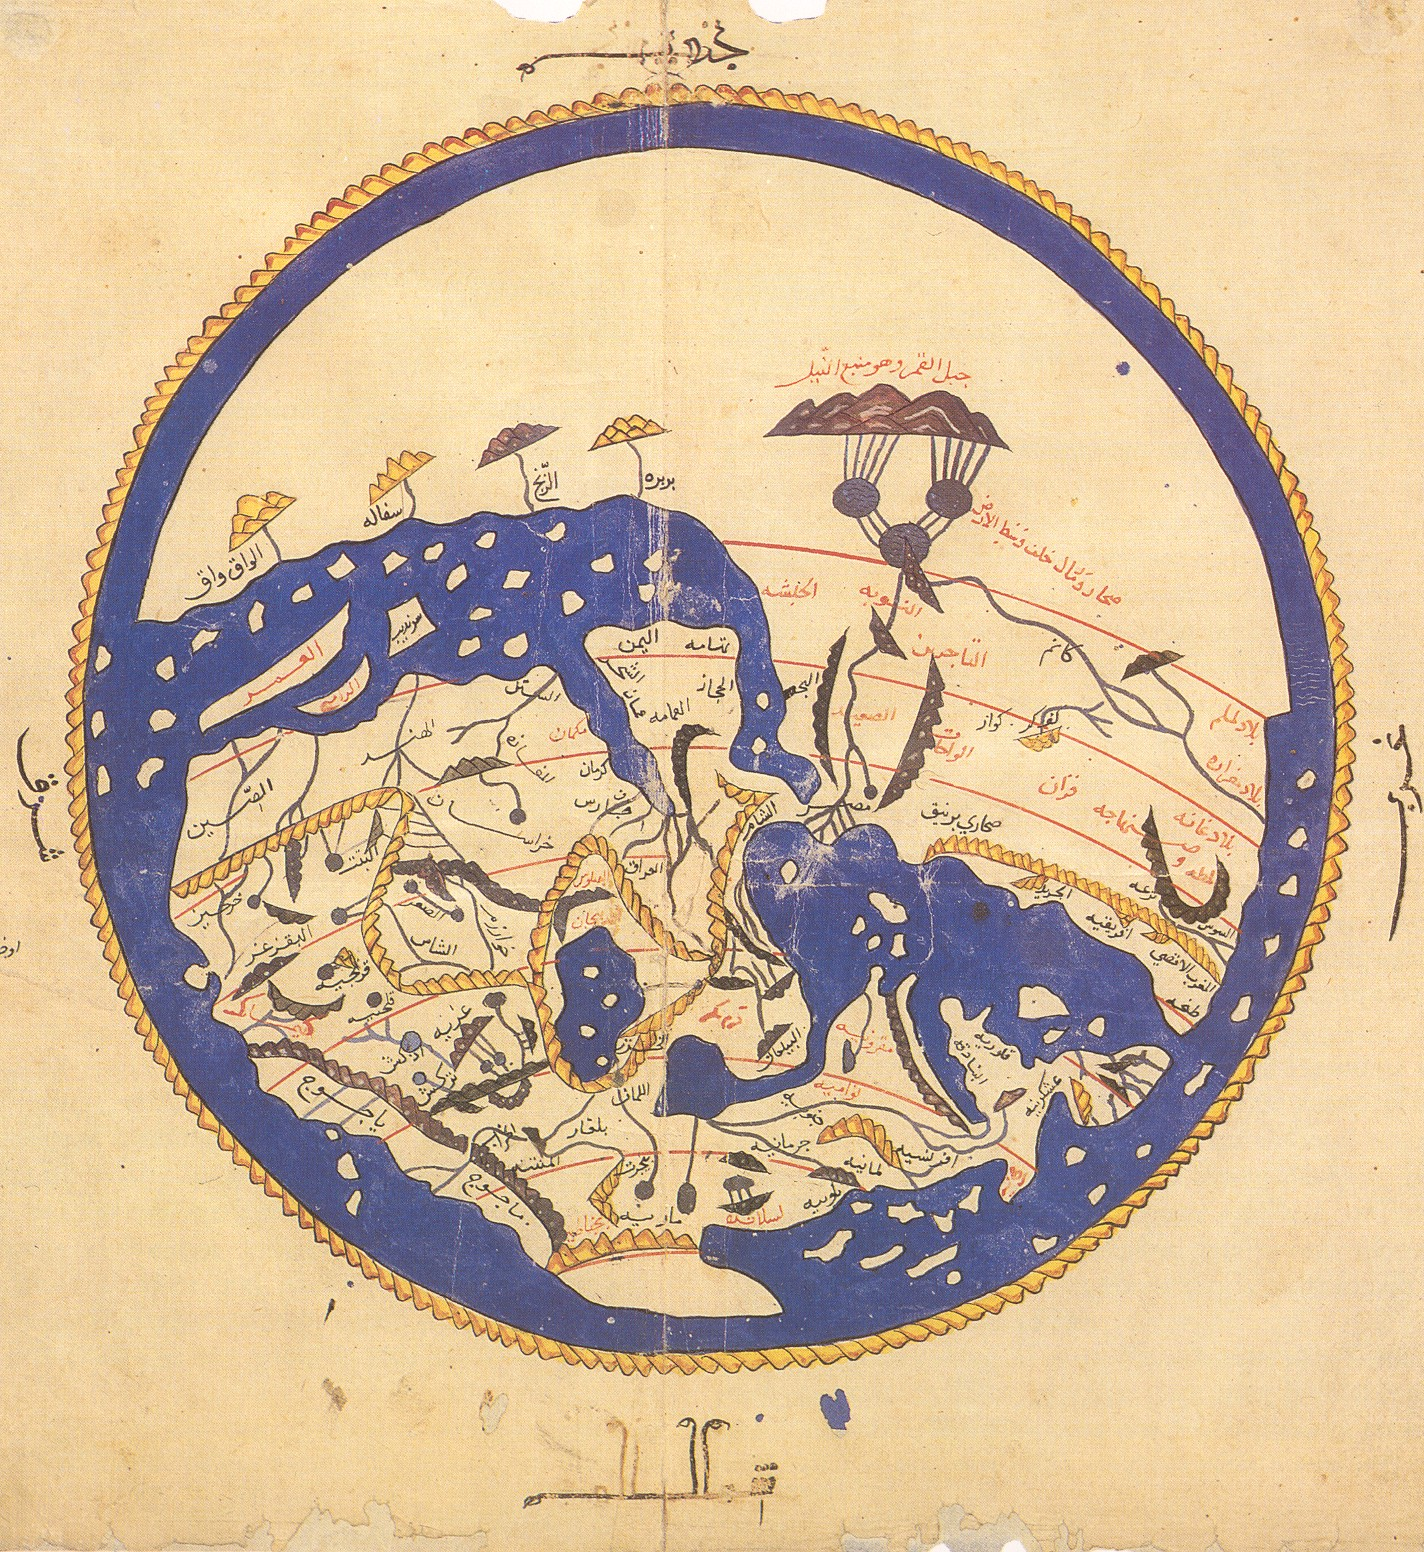
\includegraphics[width=1\textwidth]{figures/petaduniaalid.JPG}}
\caption{Gambaran pengantar peta dunia karya al-Idrisi tahun 1154.}
\end{figure}

\begin{figure}[ht]
	\centerline{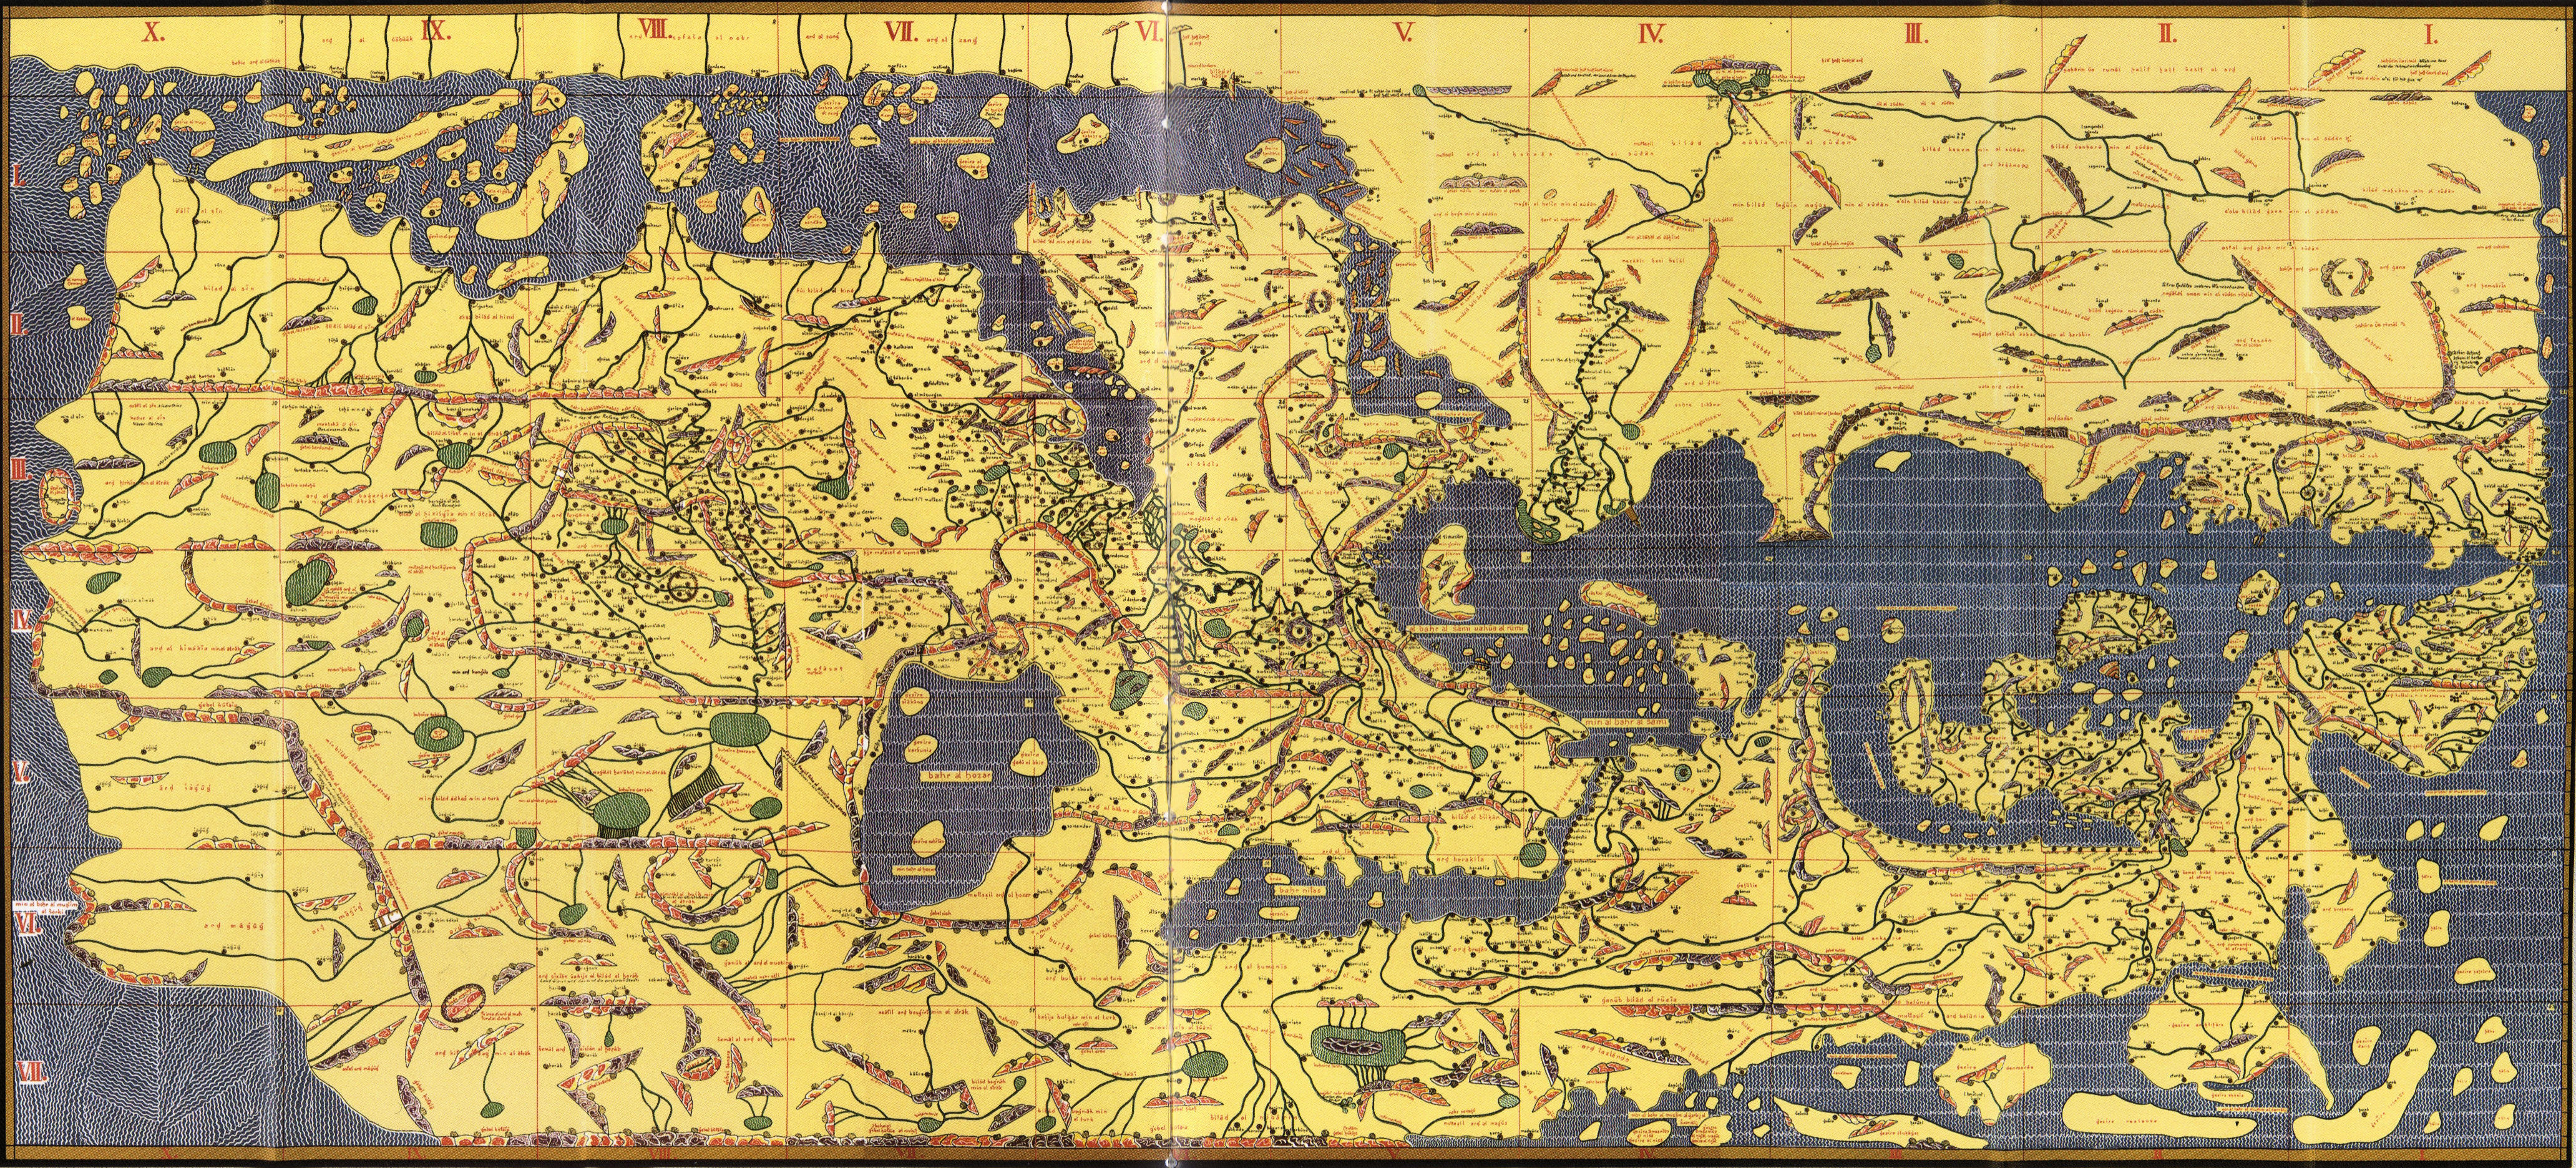
\includegraphics[width=1\textwidth]{figures/TabulaRogeriana.jpg}}
\vskip2pt
\caption{Tabula Rogeriana digambar oleh Al-Idrisi pada tahun 1154 untuk Raja Normandia Roger II dari Sisilia, setelah delapan menetap di istananya, di mana dia bekerja untuk penjelasan dan ilustrasi peta.}
\end{figure}

\section{Penentuan Kordinat}
Kordinat digunakan untuk mengacu sebuah titik lokasi di muka bumi, adapun beberapa jenis standar kordinat yang digunakan adalah.

\subsection{Kordinat Internasional}
Kordinat internasional dikenal dengan long dan lat.


\subsection{Kordinat Indonesia}
Masih ingatkah pelajaran geografi tentang letak Indonesia? maka kita bisa melihat jawaban tersebut dalam kordinat berbahasa indonesia.



\chapter[OS Semaphore]
{OS\\ Semaphore}
\section{System Operasi Semaphore}

	\subsection{Definisi}
	
		\begin{figure}[ht]
			\centerline{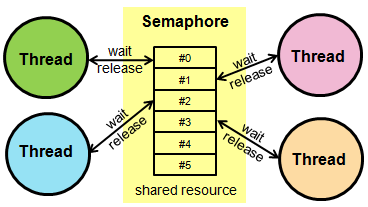
\includegraphics[width=0.5\textwidth]{figures/sema.png}}
			\caption{Semaphore}
			\label{sema}
			\end{figure}
	
		Semaphore merupakan salah satu teknik sinyal pada OS yang paling sederhana, dan merupakan konsep yang penting dalam OS desain, di mana nilai integer digunakan untuk memberi sinyal antar proses. 
		Hanya tiga operasi yang mungkin dilakukan pada semaphores, yang semuanya adalah atom: inisialisasi, keturunan, dan peningkatan. 
		Pengurangan operasi dapat menyebabkan proses yang diblokir, dan peningkatan operasi yang sedang berlangsung dapat mengakibatkan pemblokiran suatu proses. 
		Semaphore pada system operasi merupakan sebuah variabel bertipe integer. Di kehidupan nyata, semaphore merupakan sistem sinyal yang digunakan untuk memberi sinyal atau tanda dan berkomunikasi secara visual. 
		Semafor juga merupakan struktur data dalam bahasa komputer yang digunakan untuk menyinkronkan suatu proses, yaitu untuk memecahkan masalah di mana masalahnya lebih dari satu proses atau bisa 
		seperti thread yang akan dijalankan secara bersamaan dan harus diatur urutan kerja. Semaphore dibuat oleh Edsger Dijkstra dan pertama kali digunakan dalam sistem operasi.
		Nilai semaphore diinisialisasi dengan jumlah sumber daya yang dikontrol oleh pengguna. Dalam kasus khusus di mana ada sumber daya bersama, semaphore disebut semaphore biner. 
		Semaphore adalah solusi klasik dari dining philosophers problem, meskipun itu tidak mencegah deadlock.
		Pada software semaphore, semaphore merupakan variabel yang bertipe data integer tetapi tidak termasuk pada data yang sedang dilakukan inisialisasi, yang hanya dapat diakses melalui dua operasi standar, yaitu increment dan decrement. 
		Semaphore bisa digunakan untuk menyelesaikan masalah sinkronisasi secara umum, berdasarkan jenisnya. Semaphore hanya memiliki nilai 1 atau 0, atau lebih dari sama dengan 0. 
		Konsep semaphore pertama kali diajukan idenya oleh Edsger Dijkstra pada tahun 1967. Semaphore memiliki dua jenis, yaitu, Biner semaphore dan counting semaphore. 
		Biner semaphore tidak bisa memiliki semua jenis integer tetapi hanya memiliki 2 nilai yaitu 1 atau 0, Sering juga disebut sebagai semaphore primitive. Sedangkan Counting semaphore memiliki nilai 0, 1, sampai seterusnya atau integer lainnya. 
		Banyak sistem operasi yang tidak secara langsung menggunakan semaphore jenis ini, namun lebih banyak yang memanfaatkan semaphore jenis biner semaphore. 
		Pada semaphore ini harus diketahui bahwa, ada beberapa jenis dari counting semaphore yang salah satu jenisnya adalah semafor yang tidak bisa mencapai nilai negatif dan jenis yang lain adalah semaphore yang dapat mencapai nilai negatif. 
		Solusi dari Pembuatan Counting Semaphore adalah Binary Semaphore. Pembuatan counting semaphore banyak dilakukan para programmer untuk memenuhi alat sinkronisasi yang sesuai dengannya. 
		
		Operasi standarnya dalam bahasa pemrograman C :
		
		\begin{verbatim}
			void kunci(int sem_value) {
				while(sem_value <= 0);
				sem_value�;
			}
			void buka(int sem_value) {
				sem_value++;
			}
		\end{verbatim}
		
	\subsection{Prinsip Semaphore}
	
		\begin{enumerate}

			\item Suatu proses yang berbeda bisa berkaitan dengan memanfaatkan sinyal - sinyal.
			\item Suatu proses dapat dihentikan oleh proses yang lain.
			\item Semaphore bertipe data integer yang diakses oleh dua operasi atomik standar (wait dan signal).
			\item Ada dua operasi di semaphore (Down dan UP). Yang nama aslinya : P dan V.
		
		\end{enumerate}

	\subsection{Kelemahan Semaphore}
	
		\begin{enumerate}

			\item Semaphore termasuk Low Level.
			\item Dikarenakan semaphore tersebar di dalam seluruh program maka kita akan kesulitan dalam pemeliharaannya.
			\item Jika kita menghapus \"wait\" akan mengakibatkan \"nonmutual exclusion\".
			\item Jika kita menghapus \"signal\" akan mengakibatkan \"deadlock\".
			\item Jika terjadi deadlock akan sulit untuk dideteksi.

		\end{enumerate}
		
	\subsection{Semantik dan Impelementasi}
		Menghitung semaphores dilengkapi dengan dua operasi, secara historis dilambangkan sebagai P dan V (lihat § Nama operasi untuk nama alternatif). 
		Operasi V menambahkan semaphore S, dan operasi P menurunkannya.

		Nilai semaphore S adalah jumlah unit sumber daya yang saat ini tersedia. Operasi P membuang waktu atau tidur sampai sumber daya yang dilindungi oleh 
		semaphore menjadi tersedia, pada saat itu sumber daya segera diklaim. Operasi V adalah kebalikannya: ia membuat sumber daya tersedia lagi setelah proses
		selesai menggunakannya. Satu properti penting dari semaphore S adalah bahwa nilainya tidak dapat diubah kecuali dengan menggunakan operasi V dan P.

		Cara sederhana untuk memahami operasi tunggu (P) dan sinyal (V) adalah:
		
		\begin{itemize}
		
			\item menunggu: Jika nilai variabel semaphore tidak negatif, turunkan dengan 1. Jika variabel semaphore sekarang negatif, proses menunggu eksekusi 
			      diblokir (yaitu, ditambahkan ke antrian semaphore) sampai nilainya lebih besar atau sama dengan 1 Jika tidak, proses terus berjalan, setelah 
				  menggunakan satu unit sumber daya.
			\item sinyal: Menambah nilai semaphore variabel dengan 1. Setelah kenaikan, jika nilai pre-increment negatif (berarti ada proses menunggu sumber 
				  daya), ia mentransfer proses yang diblokir dari antrian menunggu semaphore ke antrean siap.
			
		\end{itemize}
		
		Banyak sistem operasi menyediakan primitif semaphore yang efisien yang membuka blokir proses menunggu ketika semaphore bertambah. Ini berarti bahwa proses tidak membuang waktu untuk memeriksa nilai semaphore yang tidak perlu.Konsep penghitungan semaphore dapat diperpanjang dengan kemampuan untuk mengklaim atau mengembalikan lebih dari satu \"unit\" dari semaphore, teknik yang diterapkan di Unix. Operasi V dan P yang dimodifikasi adalah sebagai berikut, menggunakan tanda kurung siku untuk menunjukkan operasi atom, yaitu operasi yang tampak terpisah dari perspektif proses lain:

		Semaphore pada system operasi merupakan sebuah variabel bertipe integer. Di kehidupan nyata, semaphore merupakan sistem sinyal yang digunakan untuk memberi sinyal atau tanda dan berkomunikasi secara visual. PPada software semaphore, semaphore merupakan variabel yang bertipe data integer tetapi tidak termasuk pada data yang sedang dilakukan inisialisasi, yang hanya dapat diakses melalui dua operasi standar, yaitu increment dan decrement. 
		Semaphore bisa digunakan untuk menyelesaikan masalah sinkronisasi secara umum, berdasarkan jenisnya. Semaphore hanya memiliki nilai 1 atau 0, atau lebih dari sama dengan 0. Konsep semaphore pertama kali diajukan idenya oleh Edsger Dijkstra pada tahun 1967. Semaphore memiliki dua jenis, yaitu, Biner semaphore dan counting semaphore. Biner semaphore hanya memiliki nilai 1 atau 0, Sering juga disebut sebagai semaphore primitive. Sedangkan Counting semaphore memiliki nilai 0, 1, sampai seterusnya atau integer lainnya. Banyak sistem operasi yang tidak secara langsung menggunakan semaphore jenis ini, namun lebih banyak yang memanfaatkan semaphore jenis biner semaphore

	
	\subsection{Prinsip Semaphore}
		\begin{enumerate}

			\item Suatu proses yang berbeda bisa berkaitan dengan memanfaatkan sinyal - sinyal.
			\item Suatu proses dapat dihentikan oleh proses lainnya.
			\item Semaphore bertipe data integer yang diakses oleh dua operasi atomik standar (wait dan signal).
			\item Ada dua operasi di semaphore (Down dan UP). Yang nama aslinya : P dan V.
			
		\end{enumerate}
		
	\subsection{Kelemahan Semaphore}

		\begin{enumerate}

			\item Semaphore termasuk Low Level.
			\item Dikarenaka semaphore tersebar di dalam seluruh program maka kita akan kesulitan dalam pemeliharaannya.
			\item Jika kita menghapus \"wait\" akan mengakibatkan \"nonmutual exclusion\".
			\item Jika kita menghapus \"signal\" akan mengakibatkan \"deadlock\".
			\item Jika terjadi deadlock akan sulti untuk dideteksi.
			
		\begin{enumerate}
		
	\cite{luu1982apparatus}
	\cite{lauesen1975large}
	\cite{hoare1974monitors}


\chapter[Proses OS]
{OS\\ Proses OS}
%kelompok 1 Sistem Operasi (Proses Os)
%Kelas D4 TI 1B
%Adam Noer Hidayatullah 1174097
%Ichsan Hizman
%Teddy
%Nisrina Aulia
%Irvan Rizkiansyah 1174043

\section{proses}

	\subsection{Proses}	
	Proses adalah sebuah  program yang sedang dieksekusi. Sedangkan program idalah merupakan kumpulan-kumpulan  dari suatu  instruksi yang sudah ditulis ke dalam bahasa yang dapat  dimengerti oleh sistem operasi.Proses berisi tentang sebuah instruksi dan sebuah data. program counter dan seluruh register pemroses, stack ini  berisi data sementara contohnya seperti alamat pengiriman, parameter rutin dan variabel lokal. Sistem operasi diharuskan untuk mengelola semua proses di dalam sistem tersebut dan mengalokasikan sumber daya ke sebuah  proses-proses sesuai dengan kebijaksanaan untuk memenuhi sasaran sistem
	
	\subsection{Istilah yang berkaitan dengan proses}
		\begin{itemize}
			\item Multiprogramming
			Multiprogramming (multitasking) adalah  istilah teknologi informasi dengan mengunakan bahasa inggris yang baik  mengacup kepada sebuah metode dimana banyak sebuah pekerjaan atau yang dikenal juga sebagai proses  dengan diolah dengan menggunakan sumber daya CPU yang sama.
			Contohnya sistem operasi jenis ini antaranya linux dan windows.
			\item Multiprocessing
			kemampuan komputer untuk melakukan beberapa proses dengan waktu yang bersamaan, dibantu dengan keberadaan teknologi yang berbasis multiprocessor.
			Contohnya seperti computer server.
			\item Distributed processing/computing
			Mengerjakan semua proses pengolahan data secara bersamaan antara komputer pusat dengan beberapa komputer yang lebih kecil dan saling berhubungan denan melalui jalur komunikasi.
			Contohnya komputer yang dirancang untuk melaksanakan tugas-tugas proyek.
		\end{itemize}
		
	\subsection{Fungsi fungsi sistem operasi}
		\begin{enumerate}
			\item Resource manager, pengolahan sumber daya dan mengalokasikan.
			\item Interface atau tatap muka, sebagai perantara antara pengguna dengan perangkat keras.
			\item Coordinator, mengkoordinasi fasilitas sehingga aktifitas yang komplek dapat diatur..
		\end{enumerate}
		
		\subsection{jenis jenis sistem operasi pada komputer}
			\begin{enumerate}
				\item Windows, merupakan pengembangan dari sistem operasi DOS. windows juga mudah untuk dipelajari.
				\item Mac OS, merupakan sistem operasi yang diciptakan oleh Apple. Mac OS memiliki tingkat keamanan yang tinggi.
				\item Linux, memiliki kestabilan yang baik, yang sering digunakan sebagai sistem operasi pada server.
				\item Android, merupakan sistem operasi pada smartphone. android sama seperti Linux, yaitu mudah dikembangkan.
			\end{enumerate}
			
	\subsection{Status proses}
	Terdapat 5 macam jenis status yang mungkin dimiliki oleh suatu proses :
	\begin{enumerate}
		\item New, yaitu status yang dimiliki pada saat proses baru saja terjadi.
		\item Ready, yaitu status dimana proses siap untuk dieksekusi pada giliran berikutnya.
		\item Running, yaitu status suatu proses dimana saat ini proses tersebut sedang dieksekusi oleh prosesor
		\item Waiting, yaitu status dimana proses yang tidak bisa dijalankan di saat prosesor sudah siap, status yang dimiliki pada saat proses menunggu suatu sebuah event seperti I/O
		\item Terminated, yaitu status yang dimiliki pada saat proses telah selesai dieksekusi
	\end{enumerate}
	
	Berikut ini adalah proses dari ke-5 status proses di atas :
	\begin{enumerate}
		\item New ke Ready
		Pertama Status dibuat lalu setelah itu , status akan memasuki proses ready dan siap untuk memasuki proses selanjutnya.
		\item Ready ke running
		Di saat sedang memilih proses yang akan dioperasikan, sistem operasi akan memilih salah satu proses yang berada didalam keadaan status ready.
		\item Running ke waiting
		Suatu proses dimasukkan dalam keadaan status waiting jika proses itu meminta sesuatu yang dapat menyebabkannya harus menunggu. Sebuah request ke sistem operasi yang pada umumnya merupakan bentuk panggilan dari layanan sistem (panggilan dari program yang sedang beroperasi ke dalam suatu prosedur yang merupakan bagian kode sistem operasi) misalnya seperti sebuah proses yang bisa meminta suatu layanan dari sistem operasi yang tidak siap dilakukan oleh sistem opersi dengan segera. Atau proses yang bisa menginisiasi suatu aksi, seperti misalnya operasi I/O, yang seharusnya bisa diselesaikan sebelum proses itu melanjutkan operasinya. Pada saat proses saling melakukan komunikasi dengan proses yang lainnya, suatu proses bisa diblokir jika sedang menunggu proses lainnya untuk menyediakan input.
		\item Running ke ready
		Pada umumnya alasan transisi ini ialah dimana sebuah proses yang lagi berjalan sudah mencapai batas waktu maksimum yang telah diizinkan bagi instruksi yang tidak diinterupsi. Terdapat beberapa alasan yang menyebabkan transisi ini terjadi, yang tidak diimplementasikan oleh setiap sistem operasi. Misalnya apabila sistem operasi meng-assign tingkat prioritas yang berbeda pada beberapa proses yang berlainan, suatu proses bisa diambil lebih dulu.
		\item Waiting ke ready
		Apabila suatu proses dalam keadaan status waiting sudah selesai dalam mendapatkan sumber daya, seperti file atau bagian virtual memori bagi pakai atau juga sudah selesai setelah menunggu proses yang lainnya untuk menyediakan input atau sudah selesai dalam menunggu pesan lainnya.
		\item Runing ke finish(terminated)
		proses yang sedang berjalan dihentikan oleh Sistem Operasi jika proses itu telah selesai atau tidak jadi dieksekusi. Hal ini terjadi dikarenakan jika proses induknya sendiri telah berhenti.
	\end{enumerate}
	
	Dan berikut ini adalah diagram dari ke-5 status proses tadi :
	
	\begin{figure} [ht]
	\centerline{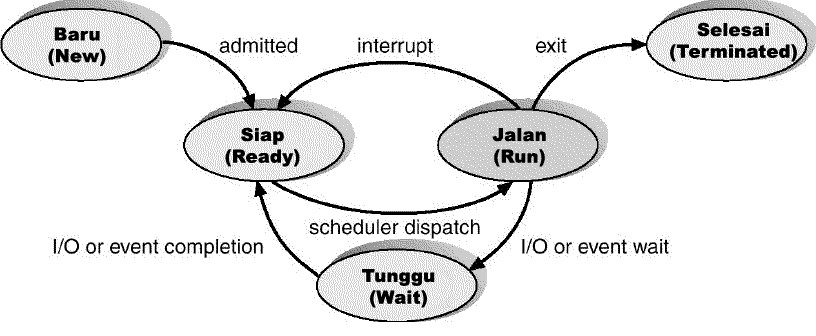
\includegraphics[width=1\textwidth]{figures/statusproses.jpg}}
	\caption{Gambar Status Proses}
	\label{statusproses}
	\end{figure}
	
	\ref{statusproses}
	
	\subsection{Contoh dari status proses}
	Setiap proses pasti mempunyai status yang harus diperhatikan oleh sistem operasi yang akan dicatat dalam berbagai macam tabel yang saling berhubungan, yaitu :
		\begin{itemize}
			\item Tabel informasi manajemen memori, Digunakan untuk menjaga keutuhan dari suatu memori utama dan memori sekunder yang akan menyimpan suatu informasi.
			\item Tabel informasi manajemen masukan atau keluaran, Digunakan untuk melakukan pengelolan sebuah perangkat masukan atau keluaran, yang dimana perangkat tersebut akan digunakan oleh proses yang tertentu, sehingga harus dijaga supaya proses yang lainnya tidak akan memakainya. Sistem operasi harus mengetahui status operasi masukan atau keluaran dan lokasi suatu memori utama yang akan digunakan untuk melakukan transfer data.
			\item Tabel informasi sistem file, Tabel dimana yang berisikan mengenai informasi lokasi pada memori sekunder, informasi ekstensi file, informasi status pada saat itu dan menyimpan atribut-atribut file yang lainnya.
			\item Tabel proses, Digunakan untuk mengelola informasi suatu proses pada sistem operasi, yang berlokasi di memori, atribut proses dan status lainnya.
		\end{itemize}
	
	\subsection{Proses Control Block/Blocked}
	Sebuah struktur data yang dipakai oleh Sistem Operasi untuk mengelola sebuah proses. Hampir semua Sistem Operasi yang modern telah menggunakan PCB (Process Control Block) namun strukturnya yang berbeda-beda pada setiap Sistem Operasi tersebut. PCB (Process Control Block) juga memiliki informasi yang berhubungan dengan proses, ialah: tanda pengenal bagi sebuah proses (Process ID) yang sangat unik dan akan menjadi status proses, nomor identitas, prioritas eksekusi proses dan semua informasi lokasi proses dalam memori. Prioritas yang dimiliki oleh sebuah proses merupakan sebuah nilai atau besaran yang akan menunjukkan seberapa sering proses harus dieksekusi oleh prosesor. Sebuah proses yang mempunyai nilai prioritas yang cenderung lebih tinggi, akan lebih sering dieksekusi atau dieksekusi terlebih dulu jika dibandingkan dengan proses yang mempunyai prioritas yang lebih rendah.
	Sebuah PCB (Process Control Block) ditunjukkan dalam tabel berikut : 
	
	\begin{table}[H]
		\begin{tabular}{|c|c|}
			\hline
			Pointer & State Proses\\
			\hline
			\multicolumn{2}{|c|}{Nomor Proses}\\
			\hline
			\multicolumn{2}{|c|}{Program Counter}\\
			\hline
			\multicolumn{2}{|c|}{Registers}\\
			\hline
			\multicolumn{2}{|c|}{Batas Memori}\\
			\hline
			\multicolumn{2}{|c|}{Daftar berkas yang telah dibuka}\\
			\hline
			\multicolumn{2}{|c|}{.......}\\
		\end{tabular}
	\end{table}
	
	PCB dibagi menjadi 3 kelompok yaitu :
	\begin{itemize}
		\item Process identification data
		pasti akan selalu mengikut-sertakan suatu identifier yang sangat unik untuk prosesnya (hampir selalu mempunyai nilai integer) dan pada sebuah sistem multiuser-multitasking, data yang contohnya seperti identifier grup pengguna, identifier proses, identifier pengguna, dan yang lainnya. Proses ini sangat relevan, karena itu sering dipakai untuk referensi silang tabel sistem operasi, misalnya seperti memungkinkan untuk mengidentifikasi sebuah proses yang menggunakan device I/O, atau daerah memori.
		\item Processor state data
		potongan-potongan dari informasi yang mengartidefinisikan status dari sebuah proses ketika proses tersebut ditangguhkan, dan memungkinkan sistem operasi untuk melakukan restart proses pada akhirnya dan akan masih dapat mengeksekusinya dengan benar. Hal ini akan selalu mengikut-sertakan isi dari register CPU tujuan.
		\item Process control data
		digunakan oleh sistem operasi untuk mengelola proses itu sendiri.
	\end{itemize}
Dirangkum dari makalah \cite{apriyanto2009sistem}
Dirangkum dari makalah \cite{silberschatz2014operating}

%\chapter[Internet]
%{Definisi\\ Internet}
%\input{section/1internet.tex}

%\chapter[Web]
%{Definisi\\ Web}
%\input{section/1web.tex}

%\chapter[Backend]
%{Definisi\\ Backend}
%\input{section/1Backend.tex}

%\chapter[Frontend]
%{Definisi\\ Frontend}
%\input{section/1Frontend.tex}

% contoh aplikasi web service
% web service
% protokol
% port

% HTTP
% URL
% POST
% GET


\bibliographystyle{IEEEtran}
\bibliography{references, kelompok31A}

\printindex

\end{document}
